\documentclass{article}
\usepackage[utf8]{inputenc}
\usepackage[english]{babel}

\usepackage{amsfonts}
\usepackage{amsthm}
\usepackage{amssymb}
\usepackage{amsmath}
\usepackage{tikz}
\usetikzlibrary{shapes.arrows,chains,trees}

\theoremstyle{definition}
\newtheorem{definition}{Definition}[section]
\newtheorem{theorem}{Theorem}[section]
\newtheorem{example}{Example}[section]

\newcommand{\G}{\mathcal{G}}

\setlength{\parindent}{0pt}

\begin{document}

\tableofcontents
\pagebreak

\section{Two problems}
Firstly we shall look at two problems which belong to the complexity class NP.

\subsection{Traveling Sales Person}
Consider a finite set $N$ of cities; $\{1, 2 \dots n\}$. The distance, or cost,
of traveling between cities $i$ and $j$ is given by $D(i,j)$ where $D$
is a symmetric matrix.

$$\forall\ i, j\quad D(i,J) \in \mathbb{N}\quad D(i,j) = D(j,i)$$

The problem is to find a path, or permutation, of
cities where each city appears exactly once in the path and the total
cost is minimised.

The brute force solution is to consider all paths, doing this would require
considering $!n$ paths.

\subsection{Boolean Formula Satisfiability}
A boolean formula consists of the logical binary operators $(\land, \lor, \neg)$
and a finite set of variables $X$ where each variable can be either true or false.
The problem consists of deciding if there exists a set of values for the variables $X$
which results in the boolean formula being true.

$$(x_1 \land x_2) \land \neg x_3$$

$$(x_1 \land x_2) \land \neg x_1$$

A brute force solution would be to consider all $2^{|X|}$ possible assignments.

The link between these two problems is the na\"ive brute force solution is not
tractable for large values of $n$.

\pagebreak
\section{Turing Machines}
What do Turing machines do? Why are we looking at them?

Conceptually a turing machine is a \textit{tape} which is infinite in both directions,
the input is writen on this tape with the rest of the tape being blank. We have a head
which can read and write to the tape. The machine moves across the tape acording to
a transition function until it reaches a terminal state which produces a yes or no result.

\begin{center}
	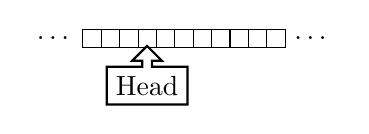
\begin{tikzpicture}[
	  start chain=1 going right,start chain=2 going below,node distance=-0.15mm
	]
		\node [on chain=1] at (-1.5,-.4) {\ldots};
		\foreach \x in {1,2,...,11} {\x, \node [draw,on chain=1] {}; }
		\node [
			name=k,
			arrow box,
			on chain=2,
			arrow box arrows={north:.25cm},
			draw=black,thick
			] at (-0.335,-1) {Head};
		\node [name=r,on chain=1] {\ldots};
	\end{tikzpicture}
\end{center}

\begin{definition}
	Formally a Turing machine consists of
	\begin{itemize}
		\item A \textit{tape alphabet} $\Gamma$ $\{a_1, a_2 \dots a_n, \beta\}$,
			where $a_i$ is a symbol, and $\beta$ is the blank or empty symbol.
		\item An \textit{input alphabet} $\Sigma$
			where $\Sigma \subset \Gamma \setminus \{\beta\}$.
		\item A set of states $Q$ $\{q_0, q_1 \dots q_m, q_y, q_n\}$ where $q_0$ is the
			initial state, $q_y$ is the terminal yes state, and $q_n$ is the terminal no state.
			$Q\prime = Q \setminus \{q_y,q_n\}$, i.e. the non-terminal states.
		\item A transition function $\delta$,
			where $\delta\ :\ (Q\prime \times \Gamma) \rightarrow
			(Q \times \Sigma \times \{L,S,R\})$.
			What this means is we look at a pair of a non-terminal state
			and a symbol from the alphabet;
			given this we enter a new state $q \in Q$,
			we write to the tape a symbol $a \in \Gamma$,
			and we stay or move the head left or right $(\{L,S,R\})$.
	\end{itemize}
\end{definition}

\begin{definition}
	Given an input $n$ and a Turing machine,
	$T(n)$ is the amount of times the transition function 
	$\delta$ must be applied to reach a terminal state.
\end{definition}

\subsection{Even or odd}
\begin{example}
	In this example we will present a turing machine to decide if a number is even.
	\begin{itemize}
		\item Input: a number $x \in \mathbb{Z}$ in unary form; i.e. $\{1 = X, 2 = XX\dots\}$,
			thus $\Sigma = \{X\}$.
		\item Output: yes iff $x$ is even, otherwise no. I.e. the turing machine will finish
			in state $q_y$ iff $x$ is even.
		\item Transition function $\delta$ is described as a matrix below with the states
			$Q\prime = \{q_0,q_1\}$ and $\Sigma = \{X,\beta\}$,
			output is $(Q \times \Sigma \times \{L,S,R\})$.
		\begin{center}
			\begin{tabular}{ c c c }
					 & $q_0$           & $q_1$           \\
				X    & ($q_1,\beta,R$) & ($q_0,\beta,R$) \\
			 $\beta$ & ($q_y,\beta,S$) & ($q_n,\beta,S$) \\
			\end{tabular}
		\end{center}
	\end{itemize}
	For this Turing machine $T(n) = n + 1$.
\end{example}

\subsection{Recognising Palindromes}

A palindrome is any word such that the reversed word is equal to the word itself,
consider the alphabet $\Gamma = \{a,b\}$, examples of palindromes would be $a, aa, aba$ etc.
Can we construct a Turing machine which recognises palindromes for the alphabet $\Gamma$?

We can, we simply move forward and backward checking each letter at opposite ends is the same,
until the entire word has been checked.
This means for palindromes $T(n)$ is equal to $n + (n - 1) \dots + 1$. Thus
$$T(n) = \frac{n^2 + n}{2}$$

However in non palindrome cases, say $aaa \dots ab$, then $T(n)$ is very small.

\subsection{Non-Deterministic Turing Machines}

\pagebreak
\section{$O, \Omega, \Theta$ Notation}

\begin{definition}
	$O(n)$
\end{definition}

\begin{definition}
	$\Omega(n)$
\end{definition}

\begin{definition}
	$\Theta(n)$
\end{definition}
Bit on worst case vs average vs best case

Note that for some $n$ $T(n)$ will be very small and for others it will be much larger,
usually this leads us to consider the complexity of the Turing machine to be 


\pagebreak
\section{Complexity class P}
\begin{definition}
	\textit{Class P} is the class of problems for which there exists a Turing machine
	which can be computed in polynomial time.
\end{definition}

\pagebreak
\section{Complexity class NP}
\begin{definition}
	\textit{Class NP} is the class of problems 
\end{definition}

\begin{theorem}
	$P \subset NP$
\end{theorem}

\begin{theorem}
	Let $\mathcal{L} \in NP$ there exist a polynomial p(n) and TM
	for solving $\mathcal{L}$ with complexity $O(2^{p(n)})$.
\end{theorem}

\pagebreak
\section{Polynomial Transformations and Equivalence}
\subsection{Polynomial Transformations}
\begin{definition}
	Consider two languages $\mathcal{L_1} \subset A_1$ and $\mathcal{L_2} \subset A_2$,
	$\mathcal{L_1}$ is said to be \textit{polynomially transformable} to $\mathcal{L_2}$ if
	$$\exists\ f : A_1 \rightarrow A_2$$
	such that $f$ can be computed with polynomially complexity and $f$ preserves the language. I.e.
	$$\forall\ x \in A_1\ x \in \mathcal{L_1}\ \mathrm{iff}\ f(x)\in \mathcal{L_2}$$
\end{definition}

Practically $\mathcal{L_1} \propto \mathcal{L_2}$ means that
$\mathcal{L_2}$ is not harder than $\mathcal{L_1}$;
i.e. if $\mathcal{L_2} \in P$ then $\mathcal{L_1} \in P$.
Furthermore this relation is transitive.
$$
  \mathcal{L_1} \propto \mathcal{L_2},\ 
  \mathcal{L_2} \propto \mathcal{L_3},\Rightarrow
  \mathcal{L_1} \propto \mathcal{L_3}
$$

\subsection{Polynomial Equivalence}
\begin{definition}
	If we have two languages such $\mathcal{L_1} \propto \mathcal{L_2}$ and
	$\mathcal{L_2} \propto \mathcal{L_1}$, then they are said to be \textit{polynomially equivalent}.
	Thus we have $\mathcal{L_1} \approx \mathcal{L_2}$.
\end{definition}
This is an equivalence as such it is reflexive, symmetric, and transitive;
as such $\forall\ R,\ S,\ T$:
\begin{itemize}
    \item $R \approx R$
    \item if $R \approx S$ then $S \approx R$.
    \item $
		R \approx S,\ 
		S \approx T \Rightarrow
		R \approx T
	$
\end{itemize}

%%TODO
In practise what this means is that we can see what problem a class is in if we can
polynomially translate it to another problem in a known class; for example:
$$
  \forall\ \mathcal{L_1} \in P\ 
  \forall\ \mathcal{L_2} \in P\ 
  \mathcal{L_1} \approx \mathcal{L_2}
$$

\section{NP-Complete problems}
\begin{definition}
	$\mathcal{L}$ is \textit{NP-Complete} if
	\begin{itemize}
		\item $\mathcal{L} \in NP$
		\item $\forall\ \mathcal{L\prime} \in NP\ \mathcal{L\prime} \propto \mathcal{L}$
	\end{itemize}
\end{definition}

What does this definition mean?
Any two NP-complete languages are polynomially equivalent.
Any NP-Complete problem is at least as hard as any other problem in NP.

\begin{theorem}
	Given two languages $\mathcal{S}, \mathcal{T} \in NP$,
	if $\mathcal{S} \in NPC$ and $\mathcal{S} \propto \mathcal{T}$ then
	$\mathcal{T} \in NPC$.
\end{theorem}

This theorem is rather useful for proving that a language is NP-Complete,
however it leaves us with the issue of proving a first language is NP-Complete.

\begin{definition}
	A boolean formula $F$ is in \textit{conjunctive normal form} if it is in the form
	\begin{equation}
	\begin{split}
		F &= f_1 \land f_2 \dots \land f_n \\
		f_i &= y_1 \lor y_2 \dots \lor y_m \\
		y_j &= x\ |\ \neg x
	\end{split}
	\end{equation}
\end{definition}

The following is in conjunctive normal form:
$$(x_1 \lor x_2) \land \neg x_3$$
The following is not in conjunctive normal form;
however it is in \textit{disjunctive normal form}
$$(x_1 \lor x_2) \lor \neg x_3$$
This is because there is the negation on the left hand side of the logical or.

\begin{definition}
	Given an undirected graph $\mathcal{G}$ which is a pair of vertices and edges $(V,E)$,
	a subset of vertices $S \subset V$ is a \textit{clique} iff
	$$\forall\ x, y \in S\ \exists\ \textrm{an edge}\ (x,y) \in E$$
\end{definition}

\begin{definition}
	If $S$ is a clique in $\mathcal{G}$ and $|S| = q$ then $S$ is called a \textit{$q$-clique}.
\end{definition}

An obvious consequence of this definition is that for any edge $(x,y)$ there is a 2-clique.

\begin{definition}
	The \textit{$q$-clique problem} is finding if there exists a $q$-clique in a given graph
	$\mathcal{G}$ where $q \in \mathbb{N}$.
\end{definition}

\pagebreak
\section{Cook’s Theorem}

\subsection{Formulation}
\begin{theorem}
    Boolean Satisfiability problem is NP-complete.
\end{theorem}
Actually we will prove that CNF-satisfiability problem is NP-complete.

\subsection{Proof}
\subsection{Formulation}
\subsection{Formulation}


\pagebreak
\section{Structure of the class NP}
\subsection{Complements to languages}
\subsection{Class co-NP}
\subsection{Some famous candidates for problems in NPI}
\subsubsection{Graph Isomorphism}
\subsubsection{Linear Programming}
\subsection{Search problems}
\subsection{Turing transformation}
\subsubsection{Informal definition}
\subsubsection{Oracle Turing Machine}
\subsubsection{Definition}

\pagebreak
\section{Approximate Algorithms}
Many problems in NP-hard are problems for which we need a polynomial algorithm;
thus we are left with few, but not none, options.
It may be the case that we can find an algorithm for our relevant cases.
Alternatively we may need to solve the problem for the input
data of a relatively small size, so that even an exponential-time algorithm is acceptable.
Finally, we can try to solve the problem approximately;
i.e. solve the problem as close to optimally as possible but accept some degree of error
or incorrectness.
This last approach is suitable for optimization search problems.

Examples of optimization search problems.
\begin{itemize}
    \item Travelling Salesperson (find the smallest tour)
    \item Find the largest clique in a graph
    \item Vertex Covering (find the smallest covering)
\end{itemize}

\subsection{Ratio bound and relative error}
For approximation algorithms we need an \textit{objective function}
which will allow us to measure the difference of the approximate and optimal algorithms.
For example in the traveling sales person problem,
the objective function is the length of the tour produced by the algorithm.
We want to determine how "close" our approximate algorithm is to the
optimal one.  We define "closeness" as \textit{ratio bound and relative error bound}.

We will assume that the objective function is always positive.

Let $C$ denote the value of the objective function at our approximate solution,
and $C\prime$ at an optimal solution.

\subsubsection{Ratio Bound}
\begin{definition}
    An approximation algorithm has \textit{ratio bound $\rho(n)$}
    if for any input of the size $n$ the value $C$ of the objective function
    at the approximate solution satisfies the inequality
    $$
    max(C/C\prime, C\prime/C) \leq \rho(n)
    $$
\end{definition}

Observe that
$$ 0 < C \leq C\prime $$
thus for maximization problems
$$ max(C/C\prime, C\prime/C) = C\prime/C $$
and for minimization problems
$$ max(C/C\prime, C\prime/C) = C/C\prime $$

Firstly observe that $\rho(n) \geq 1$,
and secondly that when $\rho(n) = 1$ we have an optimal solution.
By definition a large ratio bound (might) means that the approximate
solution is much worse than an optimal one.
This is an issue of trading speed for correctness.

\subsubsection{Relative Error Bound}
\begin{definition}
    For $C, C\prime$ and $n$  the \textit{relative error bound $\epsilon(n)$} is defined as
    $$\frac{abs(C - C\prime)}{C\prime} \leq \epsilon(n)$$
\end{definition}

Observe that $\rho(n) - 1 \leq abs(C\prime - C)/C\prime$,
i.e., $\rho(n) - 1$ is a relative error bound.

\subsection{Approximation algorithm for Vertex Covering}
\subsubsection{Vertex Covering Problem}
Recall that the vertex covering problem is defined as such
\begin{itemize}
    \item \textbf{Input}:
        a graph $\G,\ (V,E)$
    \item \textbf{Output}:
        a set $S \subset V$ such that $\forall\ (v,w) \in E$
        either $v$ or $w$ are in $S$.
        I.e. every vertex is reachable,
        and the fewest possible vertices are in $S$.
\end{itemize}

\subsubsection{Algorithm}
\begin{enumerate}
    \item Let $S$ be $\varnothing$
    \item Let $E\prime$ be the set of edges $E$
    \item While $E\prime$ is non-empty
        \begin{enumerate}
            \item
                Let $(v,w)$ be an arbitrary edge of $E\prime$
            \item
                Let $S$ be $S \cup \{v,w\}$
            \item
                Let $E\prime$ be $E\prime \setminus (v,w)$
        \end{enumerate}
    \item Return the set $S$ as the vertex covering

\end{enumerate}

\subsubsection{Properties of the Algorithm}
\begin{enumerate}
    \item The algorithm is correct
    \item The algorithm has polynomial complexity
    \item The algorithm $\rho(n) = 2$
\end{enumerate}
\textbf{Proof}
\begin{enumerate}
    \item
        The correctness is trivial
        as the algorithm simply loops until each edge has been covered.
    \item
        Polynomial time complexity is also trivial for same reason.
    \item
        Let $A$ denote the set of all edges that are chosen during the execution of the item (3) of the algorithm.
        No two edges of A have a common vertex, since once the edge (v, w) is chosen, all edges having either v or w as vertices are deleted.
        Thus, each execution of (3) adds exactly two new vertices to S and |S| = 2|A|.
        Any covering, in particular optimal $S\prime$, must cover every edge in $A$, thus any covering has at least $|A|$ vertices.
        So because we have $S\prime \supset A$ we also have
        $$|S\prime| \geq |A| = \frac{|S|}{2}$$
        $$\frac{S}{|S\prime|} \leq 2$$
\end{enumerate}

\subsection{Approximation algorithm for Travelling Salesperson with triangle inequality}
\subsubsection{$\Delta$Travelling Salesperson Problem}
The problem is formulated as such
\begin{itemize}
    \item \textbf{Input}:
        A matrix $d_{ij}$ such that $\forall\ i,j\, d(i,j) > 0$
        $$
        i,j,k d(i,j) \leq d(i,k) + d(k,j)
        $$
    \item \textbf{Output}:
        A tour such that every 
\end{itemize}

\subsubsection{Algorithm for $\Delta$Traveling Salesperson}
Given a connected graph $\mathcal{G}\ (V,E)$,
\begin{enumerate}
    \item
        Choose a vertex $v \in V$, to serve as the root of a tree.
        Build a spanning tree $T$ beginning at $v$;
        note that this can be done in polynomial time using Prim's or Kruskal's algorithm.
    \item
        Perform a pre-order walk on the tree $T$ returning the list of nodes as a tour.
\end{enumerate}

We can now propose three properties of this algorithm
\begin{enumerate}
    \item It is correct
    \item It has polynomial complexity
    \item It has a ratio bound $\rho(n) = 2$
\end{enumerate}
\textbf{Proof}
\begin{enumerate}
    \item
        The correctness is trivial
    \item
        Proof of polynomial complexity is trivial.
    \item
        The ratio bound
\end{enumerate}

\pagebreak
\section{Complexity Lower Bounds}
\begin{definition}
    A function $L(n)$ is called a \textit{complexity lower bound}
    for a computational problem $L$
    in a given class $M$ of models of computation
    if for any algorithm from $M$ which solves $L$ with complexity $T(n)$ the following relation holds:
    $$T(n) = \Omega(L(n))$$
\end{definition}

Finding non-trivial lower bounds is an important part of a comprehensive analysis of an algorithm,
which might save time spent on trying to construct a better algorithm.
Very few natural problems have proven lower bounds in the class of all Turing machines because these models are powerful.
An example of the quadratic lower bound for the problem of recognizing palindromes in the class of one-tape,
one-head Turing machines was mentioned earlier in this unit.
If we assume $P \neq NP$ hypothesis, then any polynomial serves as a lower bound for any NP-complete problem in the class of all Turing machines.
Clearly it should be easier to prove lower bounds for narrower classes $M$ of algorithms.
On the other hand such a class should be “natural enough” for the lower bound to be of some practical use.
This part of Lecture Notes describes a general method for proving complexity lower bounds for algebraic computation trees.

\subsection{A Lower Bound for Comparison Sorting}
We can arrive at a lower bound for comparison based for sorting using decision trees.

As input we have a finite set of items to sort
and a binary relation $\leq$ where we have $\forall\ a,b,c:$
\begin{itemize}
    \item Reflexivity: $a \leq a$
    \item Anti-Symmetry: if $a \leq b$ and $b \leq a$ then $a = b$
    \item Transitivity: if $a \leq b$ and $b \leq c$ then $a \leq c$
\end{itemize}

\begin{example}
The most obvious example is less than equal on the integers
$$1 \leq 1 \leq 2 \leq 74782$$
$$1 \leq 74782$$
\end{example}

We will use any given binary relation as the basis of our decision tree,
at each node of the tree we compute one binary relation
the left child will represent the result of the computation being true
conversely the right child will mean the computation result was false.
$$$$
Consider sorting three items $(a,b,c)$ we can derive a decision tree showing that
there exists a lower bound complexity for comparison sorting.

\begin{center}
    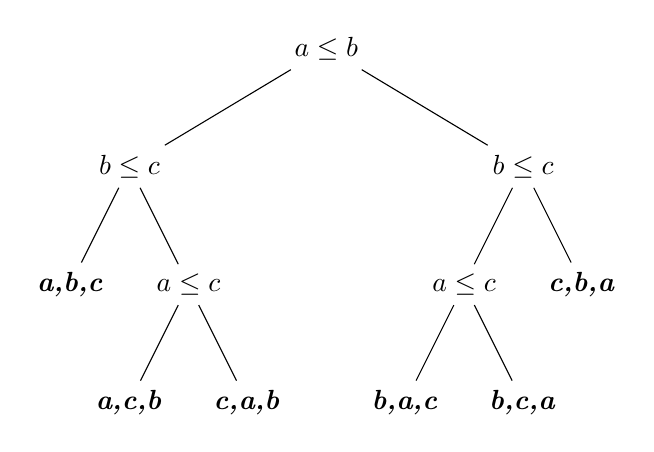
\begin{tikzpicture}[level distance=1.5cm,
  level 1/.style={sibling distance=5cm},
  level 2/.style={sibling distance=1.5cm},
  level 3/.style={sibling distance=1.5cm}]
  \node {$a \leq b$}
    child {node {$b \leq c$}
        child {node {\textbf{\textit{a,b,c}}}}
        child {node {$a \leq c$} {
          child {node {\textbf{\textit{a,c,b}}}}
          child {node {\textbf{\textit{c,a,b}}}}
      }}
    }
    child {node {$b \leq c$}
        child {node {$a \leq c$} {
          child {node {\textbf{\textit{b,a,c}}}}
          child {node {\textbf{\textit{b,c,a}}}}
      }}
          child {node {\textbf{\textit{c,b,a}}}}
    };
\end{tikzpicture}
\end{center}

Observe that the height or depth of the tree represents the amount of computations which must be performed.
Furthermore observe that the height of the tree is not the same for every root,
for the ordering \textbf{\textit{b,a,c}} we have height three
and for \textbf{\textit{a,b,c}} we have height two.
This is because we can prune some branches due to the transitive property of $\leq$,
given $a \leq b$ and $b \leq c$ we also know that $a \leq c$ is true.
Thus we do not need to compute $a \leq c$.
Conversely given $a \leq b$ and $c \leq b$ we \textbf{do not know} that $a \leq c$ is true.
This is another computation we need to perform to have a correct ordering.
Obviously this tree is correct for $n = 3$, so we can say
the complexity lower bound for $n = 3$ is 3 computational steps.
This is because equipped with only comparison we can only go in one
of two directions after each computation (true or false),
and we must be able to produce all six possible orderings.

How do
How many branches can we prune?

Well for a three item set $(a,b,c)$ there exists precisely $!3 = 6$ orderings;
thus our decision tree 
or more generally there exists for an $n$ item set $!n$ orderings.
Because
$$\Omega(n log n)$$


\subsection{Algebraic computation trees: examples}
We can expand the decision tree model to something more powerful

Consider the problem of finding if a point is inside the unit circle
\begin{itemize}
    \item Input: a point $(x,y) \in \mathbb{R}^2$
    \item Output: yes iff $x^2 + y^2 \leq 1$
\end{itemize}
The complexity of this algorithm (the height of the tree) is 4, i.e., a constant.
This is quite natural since we assume that the size of the input is a constant.
\begin{center}
    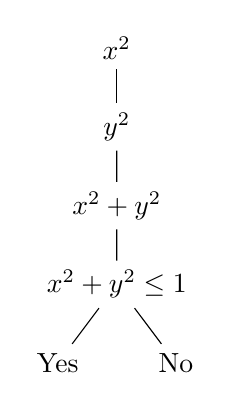
\begin{tikzpicture}[level distance=1cm,
  level 1/.style={sibling distance=2cm},
  level 2/.style={sibling distance=1.5cm},
  level 3/.style={sibling distance=1.5cm},
  level 4/.style={sibling distance=1.5cm},
  level 5/.style={sibling distance=1.5cm}]
  \node {$x^2$}
        child {node {$y^2$}
        child {node {$x^2 + y^2$}
        child {node {$x^2 + y^2 \leq 1$}
            child {node {Yes}}
            child {node {No}}
            }}
        };
\end{tikzpicture}
\end{center}

To further generalise our algebraic computation trees,
we will say that every node, except leaves, have three children.
The children correspond to the computation being
\begin{enumerate}
    \item $(= 0)$
    \item $(< 0)$
    \item $(> 0)$
\end{enumerate}
In the example below for the sake of space and brevity we don't show all the different branches,
simply because we never make any changes to our computation dependent on the result;
that is until the very end where we use it for our yes or no result.
This tree, were it completed, would have $3^4 = 81$ nodes,
much more than our previous tree.
However observe that the height remains unchanged at four,
thus the complexity is the same.

\begin{center}
    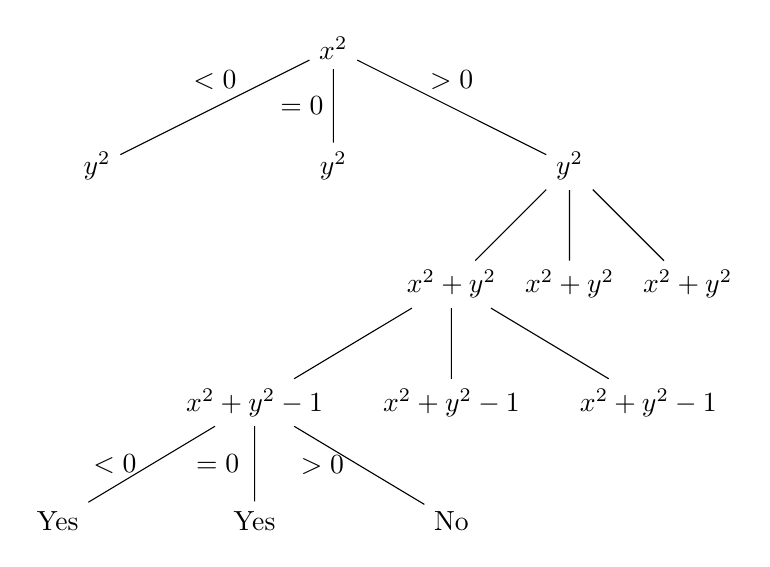
\begin{tikzpicture}[level distance=1.5cm,
  level 1/.style={sibling distance=3cm},
  level 2/.style={sibling distance=1.5cm},
  level 3/.style={sibling distance=2.5cm},
  level 4/.style={sibling distance=2.5cm}]
    \node {$x^2$}
            child {node {$y^2$} edge from parent node[left,above=3pt] {$< 0$}
            }
            child {node {$y^2$} edge from parent node[left] {$= 0$}
            }
            child {node {$y^2$}
                child { node {$x^2 + y^2$} 
                    child { node {$x^2 + y^2 - 1$} 
                        child { node {Yes} edge from parent node[left=2pt] {$< 0$}}
                        child { node {Yes} edge from parent node[left=2pt] {$= 0$}}
                        child { node {No}  edge from parent node[left=2pt] {$> 0$}}
                    }
                    child { node {$x^2 + y^2 - 1$} }
                    child { node {$x^2 + y^2 - 1$} }
                }
                child { node {$x^2 + y^2$} }
                child { node {$x^2 + y^2$} }
            edge from parent node[left,above=3pt] {$> 0$} }
       ;
\end{tikzpicture}
\end{center}

\begin{example}
    One can generalise this example from membership of the unit circle to membership
    of the $n$ dimensional unit ball.
    Simply calculate
    $$1 \leq \sum_{i=1}^{n} x_i^2$$
    You calculate $x_i^2$ for the $i$-th dimension and add it to the running total;
    this takes $2n$ steps.
    In case $n = 2$ we get complexity four as our computation tree showed.
\end{example}

\subsection{Algebraic computation trees: definition}
\begin{definition}
    A subset $S \subset R^n$ is called \textit{(basic) semi-algebraic} if it is defined by
    $$\{P_1(x_1,\dots x_n) = 0,\dots P_n\}
    \cup
    \{Q_1(x_1,\dots x_n) > 0,\dots Q_m\}$$
    where $P_i$ and $Q_j$ are polynomials in $n$ variables
    i.e., S is a set of all solutions of a system of equations and strict inequalities.
\end{definition}

Algebraic computation tree $T$ in variables $x_1,\dots x_n$
is a tree with the root $v_0$ such that to every vertex $v$ (except leaves)
is an arithmetic operation (addition, subtraction or multiplication) 
and a polynomial $f_v$ is attached.

For example $f_3 = f_1 + f_2$ where $f_3$ is the new polynomial;
more precisely in our previous example membership of the unit circle
we have
$$f_1 = x^2 \quad f_2 = y^2 \quad f_3 = x^2 + y^2$$
$$f_4 = f_3 - 1 = x^2 + y^2 - 1$$

Let $v_0, v_1,\dots, v_\omega$ be the sequence of vertices
along the (unique) branch leading from the root $v_0$ to $v_\omega$.
An arithmetic operation at $v_i$ is performed on a pair from
$$\{x_1,\dots x_n\} \cup \{f_0\dots f_{i - 1}\}$$
and the result is at $f_i$.
Note that every $v$ has exactly three children
$$(> 0, = 0, < 0)$$

Let $*_i \in \{>0,=0,<0\}$ for $0 \leq i < \omega$ be the sign of $f_{v_i}$,
One can assign the semi-algebraic set $U_\omega$ to $v_\omega$
$$U_\omega = \{f_0*_00,f_1*_10\dots f_{\omega - 1} *_{\omega - 1}0\}$$

To each leaf $\omega$ of $T$ an output Yes or No is assigned.
We call $U_\omega$ an accepting set if the leaf $\omega$ has the output Yes assigned.
We say that T tests the membership to the union of all accepting sets.

The computation process works as follows.
A specific point $x \in \mathbb{R}^n$ is taken as an input.
Then the value $f_{v_0}(x)$ is computed and the sign of this value is determined.
According to the sign, the algorithm goes to the corresponding child $v_1$ of $v_0$.
If the process eventually arrives to a Yes-vertex, then $x$ belongs to an accepting set,
and, therefore, to the union of all accepting sets.

\subsection{Distinctness problem: upper bound}
\begin{itemize}
    \item \textbf{Input:} $(x_0, x_1,\dots x_n) \in \mathbb{R}^n$
    \item \textbf{Output:} Yes iff $\forall\ i,j$ where $0 \leq i,j \leq n, i \neq j$ we have $x_i \neq x_j$
\end{itemize}
An immediate solution for this problem is to sort the numbers $(x_0, x_1,\dots x_n)$
then compare pairwise neighbours for equivalence; this has complexity $O(nlogn)$.
It is clear that this algorithm can be represented in a form of algebraic computation tree
of the height $O(nlogn)$ (compare with sorting).
We are going to develop a general method for proving lower complexity bounds for algebraic computation trees,
and will apply this method to prove the $\Omega(nlogn)$ lower bound for Distinctness.
Unlike the very elementary proof of $\Omega(nlogn)$ for sorting,
for Distinctness no elementary proof is known.

\subsection{Connected components of semialgebraic sets}
Informally, a finite union $W$ of semialgebraic sets is called connected
if for every $x, y \in W$ there is a “continuous” curve in $W$ containing both $x$ and $y$.
A formal definition can be found in textbooks on topology.

\begin{definition}
    Any maximal (with respect to the set-theoretical inclusion) connected subset of W is called connected component of W.
\end{definition}

\begin{theorem}
    Every finite union W of semialgebraic sets can be uniquely represented as a union of a finite number of its connected components:
    $$W = \bigcup\limits_{1\leq i \leq k} W_i$$
    which are finite unions of semialgebraic sets.
\end{theorem}

\begin{example}
    Consider these examples of
    \begin{enumerate}
        \item The union %of open intervals W = (0, 1) ∪ (2, 3) ⊂ R is not connected. Intervals (0, 1) and (2, 3) are connected components of W .
        \item The union %W = (0, 1) ∪ (1, 2) is not connected with (0, 1), (1, 2) being W ’s connected components.
        \item The union %W = (0, 1) ∪ 1 ∪ (1, 2) = (0, 2) is connected and is its own unique connected component.
        \item The semialgebraic set %W = {X ̸= Y } ⊂ R2 (which also can be written in the form W = {X2 − 2XY + Y 2 > 0}) is not connected and has two connected components: {X − Y > 0} and {Y − X > 0}.
    \end{enumerate}
\end{example}

\begin{theorem}
    Projection %of a connected set W ⊂ Rn+m on a coordinate subspace Rn is also connected.
\end{theorem}

\subsection{Lower bound for membership to a semialgebraic set: decision computation trees}
\subsection{Thom-Milnor’s bound}
\subsection{Lower bound for membership to a semialgebraic set: algebraic computation trees}
\subsection{Distinctness problem: lower bound}

\pagebreak
\section{Complexity and Quantum Computing}
\subsection{Complex Numbers}
\subsection{Vectors and matrices}
\subsection{Qubits}
\subsection{Bloch sphere}



\end{document}
